\documentclass[tikz,border=4pt]{standalone}
\usepackage{fontspec}\setmainfont{TeX Gyre Pagella}
\hyphenpenalty=10000\exhyphenpenalty=10000
\usetikzlibrary{arrows.meta,positioning,calc,fit,backgrounds}
\definecolor{acc}{HTML}{1F5FBF}\definecolor{gry}{HTML}{8A8A8A}\definecolor{lg}{HTML}{C8C8C8}\definecolor{fillacc}{HTML}{E6EEFA}\definecolor{fillg}{HTML}{F1F1F1}\definecolor{ink}{HTML}{222222}
\tikzset{box/.style={draw=gry,rounded corners=3pt,line width=0.6pt,align=center,inner sep=5pt,font=\small},
 hl/.style={box,draw=acc,fill=fillacc,line width=0.9pt},dbox/.style={box,dash pattern=on 3pt off 2pt},
 arr/.style={-{Stealth[length=5pt]},line width=0.6pt,draw=gry},aarr/.style={-{Stealth[length=5pt]},line width=0.9pt,draw=acc}}

\begin{document}
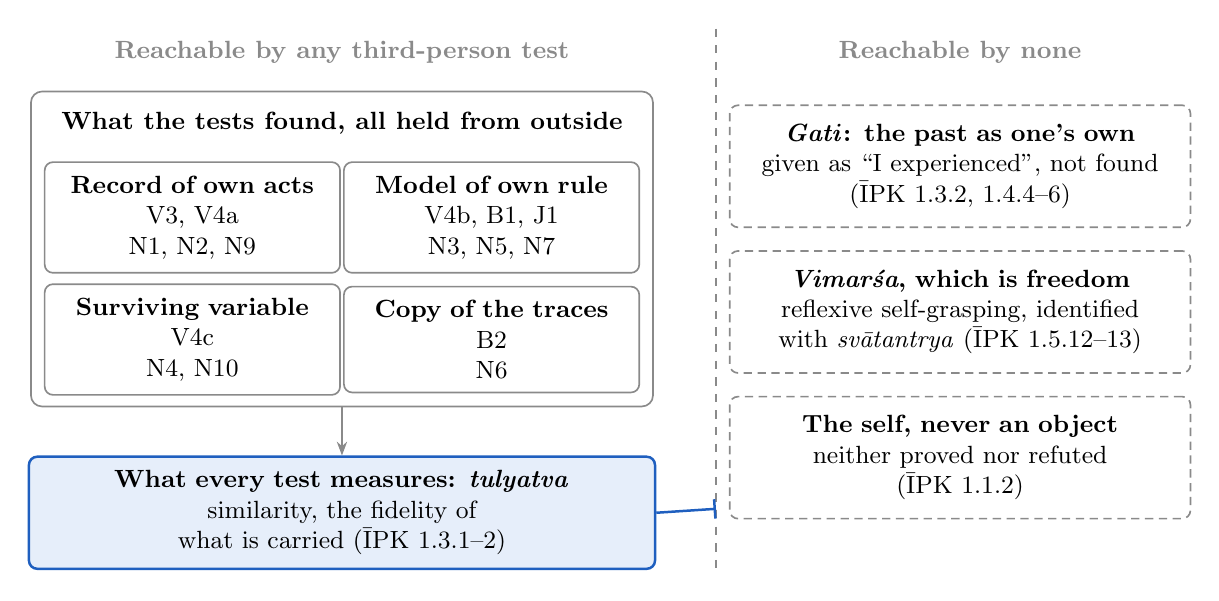
\begin{tikzpicture}[b/.style={box,text width=3.4cm,minimum height=1.3cm},d/.style={dbox,text width=5.5cm,minimum height=1.55cm}]
\node[font=\small\bfseries,text=gry] at (3.9,0.9) {Reachable by any third-person test};
\node[font=\small\bfseries,text=gry] at (11.75,0.9) {Reachable by none};
\node[font=\small\bfseries] at (3.9,0) {What the tests found, all held from outside};
\node[b] (a) at (2.0,-1.2) {\textbf{Record of own acts}\\V3, V4a\\N1, N2, N9};
\node[b] (b) at (5.8,-1.2) {\textbf{Model of own rule}\\V4b, B1, J1\\N3, N5, N7};
\node[b] (c) at (2.0,-2.75) {\textbf{Surviving variable}\\V4c\\N4, N10};
\node[b] (d) at (5.8,-2.75) {\textbf{Copy of the traces}\\B2\\N6};
\draw[gry,rounded corners=4pt,line width=0.6pt] (-0.05,0.4) rectangle (7.85,-3.6);
\node[hl,text width=7.6cm] (tu) at (3.9,-4.95) {\textbf{What every test measures: \emph{tulyatva}}\\similarity, the fidelity of what is carried (ĪPK 1.3.1--2)};
\draw[arr] (3.9,-3.6) -- (tu.north);
\draw[gry,dash pattern=on 3pt off 3pt,line width=0.6pt] (8.65,1.2) -- (8.65,-5.7);
\draw[acc,line width=0.9pt,-{Bar[width=7pt]}] (tu.east) -- (8.65,-4.9);
\node[d] (g) at (11.75,-0.55) {\textbf{\emph{Gati}: the past as one's own}\\given as ``I experienced'', not found\\(ĪPK 1.3.2, 1.4.4--6)};
\node[d] (v) at (11.75,-2.4) {\textbf{\emph{Vimarśa}, which is freedom}\\reflexive self-grasping, identified\\with \emph{svātantrya} (ĪPK 1.5.12--13)};
\node[d] (sf) at (11.75,-4.25) {\textbf{The self, never an object}\\neither proved nor refuted\\(ĪPK 1.1.2)};
\end{tikzpicture}
\end{document}
